

\begin{frame}{Introduction}

  \begin{block}{PASC Project: GeoPC (2013-2016)}
  \begin{itemize}
   \item Infrastructure development for hybrid parallel smoothers for multigrid preconditioners
   \item Today's topic: GPU acceleration for SpMV
   \item More results: MS8, 17:00-17:30, Room C2-3
  \end{itemize}
  \end{block}

    \begin{center} \vspace*{2cm}
    
\includegraphics[width=0.3\textwidth]{figures/pasc}
  \end{center}

\end{frame}




\begin{frame}{pTatin3d}
   \begin{center} \Large \textbf{GPU-SpMV in pTatin3d} \end{center}
\end{frame}



% About pTatin3d


\begin{frame}{pTatin3d}

  \begin{block}{About pTatin3d}
  \begin{itemize}
   \item Geodynamics modeling package
   \item Simulates long-term lithospheric deformation
   \item Solves heterogeneous Stokes problems
  \end{itemize}
  \end{block}

  \begin{block}{Discretization and Solver}
  \begin{itemize}
   \item Inf-sub stable $Q_2-P_1^{\mathrm{disc}}$ elements
   \item (F)GMRES with multigrid preconditioner
   \item Matrix-free application of viscous block
  \end{itemize}
  \end{block}

\end{frame}


% Solver Setup
\begin{frame}{pTatin3d}

  \begin{block}{Equations in $\Omega$}
        \begin{align*}
          \nabla \cdot \bigl[ 2 \eta(\mathbf u, p) \mathbf D(\mathbf u) \bigr] - \nabla p &= \mathbf f \ , \quad \mathrm{where} \ 
          \mathbf D(\mathbf u) := \frac{1}{2}\bigl(\nabla \mathbf u^{\mathrm T} + \nabla \mathbf u \bigr) \ , \\
          \nabla \cdot u &= \mathbf 0
         \end{align*}
  \begin{itemize}
   \item Fluid velocity $\mathbf u$, pressure $p$
   \item Effective shear viscosity $\eta$
   \item Body force $\mathbf f$
  \end{itemize}
  \end{block}

  \begin{block}{Boundary Conditions}
  \begin{itemize}
   \item \ \ \ \ $\, \, \! \mathbf u = \mathbf{\overline{u}}$ on $\Gamma_{\mathrm D}$ (Dirichlet)
   \item $\mathbf u \cdot \mathbf n = \mathbf{\overline{t}}$ on $\Gamma_{\mathrm N}$ (Neumann)
  \end{itemize}
  \end{block}

  \begin{flushright}
   \vspace*{-4cm} 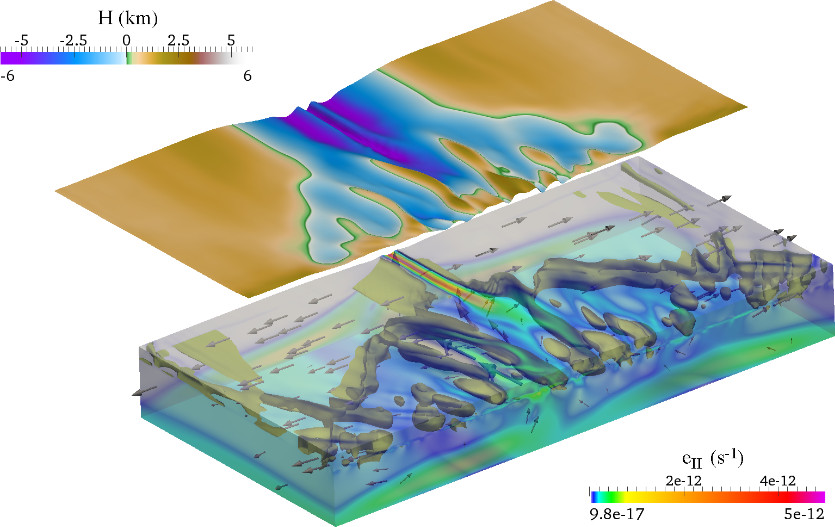
\includegraphics[width=0.45\textwidth]{figures/rifting} \\
   {\scriptsize (D.~May, J.~Brown, L.~Le Pourhiet, 2014)}
  \end{flushright}

\end{frame}


\begin{frame}{pTatin3d}

  \begin{block}{Field-Split for Nonlinear System}
        \begin{align*}
          \left[ \begin{array}{cc} \mathbf{J}_\mathrm{uu}  &  \mathbf{J}_\mathrm{up} \\
                                   \mathbf{J}_\mathrm{pu}  &  \mathbf 0
                 \end{array} \right]
                 = - \left[
                 \begin{array}{c}
                  \mathbf F_u \\
                  \mathbf F_p
                 \end{array} \right]
         \end{align*}
  \begin{itemize}
   \item $\mathbf{J}_\mathrm{uu}$ symmetric, positive definite
   \item Schur complement $\mathbf{S} = -  \mathbf{J}_\mathrm{pu}  \mathbf{J}_\mathrm{uu}^{-1} \mathbf{J}_\mathrm{up}$ (expensive)
  \end{itemize}
  \end{block}
  
  %\pause
  \begin{block}{Approximate Preconditioner}
    \begin{align*} \mathbf P = \left[
      \begin{array}{cc}
        \tilde{\mathbf{J}}_\mathrm{uu}  &  \mathbf 0 \\
               \mathbf{J}_\mathrm{pu}  &  \tilde{\mathbf S}
      \end{array} \right]
    \end{align*}
   \begin{itemize}
    \item Multigrid for $\tilde{\mathbf{J}}_\mathrm{uu} := \mathbf{J}_\mathrm{uu}$ with Jacobi-preconditioned Chebychev-smoother
    \item Scaled mass-matrix for $\tilde{\mathbf S}$
   \end{itemize}

  \end{block}


\end{frame}

% GPU optimization steps


\begin{frame}{pTatin3d}

  \begin{block}{Matrix-free Application of $\mathbf{J}_\mathrm{uu}$}
  \begin{itemize}
   \item Use hierarchical tensor basis for $Q_2$ elements on hexahedra:
    \begin{align*}
     A\mathbf{u} = \sum_{\mathrm{elements}\ e} \mathcal{E}_e^{\mathrm T} D_\xi^{\mathrm T} \Lambda\Bigl( (\nabla_{\mathbf x} \xi)^{\mathrm T} (\omega \eta) (\nabla_{\mathbf x} \xi) \Bigr) D_\xi \mathcal{E}_e  \mathbf{u}
    \end{align*}
   \item Reference derivative matrix $D_\xi$ composed of $\hat{D} \otimes \hat{B} \otimes \hat{B}$, $\hat{B} \otimes \hat{D} \otimes \hat{B}$, and $\hat{B} \otimes \hat{B} \otimes \hat{D}$
   \item Higher FLOP/Byte ratio and lower memory bandwidth requirements
  \end{itemize}
  \end{block}

  %\pause
  \begin{block}{Previous Work: AVX-Vectorization}
   \begin{itemize}
    \item Vectorize over elements: 4 elements per AVX register (double precision, 256 bits)
    \item Details: May \textit{et al.}, SC14 (2014)
   \end{itemize}

  \end{block}
  
\end{frame}




% Performance modeling (kernel)

\begin{frame}{pTatin3d}

  \begin{block}{GPU-accelerated SpMV, First Attempt}
  \begin{itemize}
   \item One thread per element
   \item Same execution flow as CPU version
   \item Updates to result postponed and computed on host
  \end{itemize}
  \end{block}

  %\pause
  \begin{block}{Observations}
   \begin{itemize}
    \item It works!
    %\pause
    \item It's relatively slow (excessive register spilling)
   \end{itemize}
  \end{block}
  
\begin{center}
\begin{tabular}{|c|c|c|c|}
 \hline
 mx=my=mz        & AVX (1 proc) & CUDA & OpenCL \\
 \hline
 \hline
 16              &  4.0         &  2.6  &  3.2  \\
 24              & 11.1         &  4.9  &  5.4  \\
 32              & 54.6         & 22.0  & 25.3 \\
 48              & 131.5        & 59.5  & 65.3  \\
 \hline
\end{tabular} \\
(Timings in seconds, Piz Daint prior to upgrade)
\end{center}
  
\end{frame}


\begin{frame}{pTatin3d}

  \begin{block}{GPU-accelerated SpMV, Optimizations}
  \begin{itemize}
   \item Stash GPU data to reduce host-device communication
   \item Use one warp per element
   \item Concurrent writes to result vector via atomics or coloring
   \item CUDA: Use warp shuffles for tensor computations
  \end{itemize}
  \begin{flushright} \vspace*{-2.5cm}
    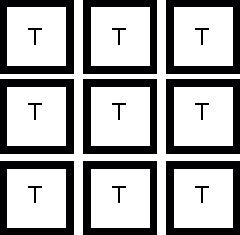
\includegraphics[width=0.15\textwidth]{figures/threads-before} \ \ \ 
    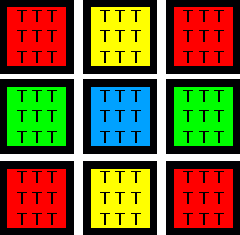
\includegraphics[width=0.15\textwidth]{figures/threads-after}
  \end{flushright}
  \end{block}

   %\pause
  \begin{block}{Observations}
   \begin{itemize}
    \item GPU occupancy at 25 percent (enough to cover memory latencies)
    \item 166 GFLOPs (70 percent of 235, one FLOP per 4 warp shuffles)
   \end{itemize}
  \end{block}
  
\begin{center}
\begin{tabular}{|c|c|c|c|}
 \hline
 mx=my=mz        & AVX (1 proc) & CUDA, unoptimized & CUDA, optimized \\
 \hline
 \hline
 16              &  4.0         &  2.6  &  1.0  \\
 24              & 11.1         &  4.9  &  2.2  \\
 32              & 54.6         & 22.0  &  8.1  \\
 48              & 131.5        & 59.5  & 14.6  \\
 \hline
\end{tabular} \\
(Timings in seconds, Piz Daint prior to upgrade)
\end{center}
  
\end{frame}


% Performance modeling (multigrid)


\begin{frame}{pTatin3d}

  \begin{block}{Profiling Data for SpMV within Multigrid (Dual Xeon E5-2620 with Tesla K20)}
  \begin{itemize}
   \item Setup for SpMV (Gauss data, etc.): $<$1 percent
   \item Copy field data: 21 percent
   \item Kernel execution: \textbf{23 percent}
   \item Copy result: 16 percent
   \item Other (boundary conditions, etc.): 39 percent
  \end{itemize}
  \end{block}

  
\begin{center} \footnotesize
\renewcommand{\arraystretch}{1.4}
\begin{tabular}{|c||c|c|c||c|c|}
 \hline
 mx=my=mz        & AVX (1T)      & AVX (2x12T)  & AVX (12x2T) & CUDA          & OpenCL \\
 \hline
 \hline
 16              &  4.7s / 7.1 &   2.4s / 14.0  & 0.7s / 52.8  &  1.0s / 33.6  & 1.1s / 30.5 \\
 24              & 12.8s / 6.9 &   4.3s / 20.4  & 1.5s / 62.4  &  2.2s / 40.0  & 2.4s / 36.7 \\
 32              & 49.2s / 6.8 &  16.4s / 20.6  & 4.3s / 66.0  &  8.1s / 40.7  & 8.2s / 40.2 \\
 40              & 55.4s / 6.9 &  16.5s / 23.1  & 6.1s / 69.6  &  9.3s / 40.9  & 9.4s / 40.4 \\ 
 48              & 82.3s / 6.9 &  22.5s / 25.1  & 8.7s / 68.4  & 14.6s / 38.7  & 15.2s / 37.1 \\
 \hline
\end{tabular} \\
 Time/GFLOPs
\end{center}

\end{frame}







\begin{frame}{StagYY}
  \begin{center} \Large \textbf{GPU-assisted Multigrid in StagYY} \end{center}
\end{frame}




% About StagYY


\begin{frame}{StagYY}

  \begin{block}{About StagYY}
  \begin{itemize}
   \item Mantle convection solver
   \item Cartesian, 3D spherical shell, cylindrical domains
   \item Further details: P.~Tackley, J. PEPI (2008)
  \end{itemize}
  \end{block}

  \begin{block}{Discretization and Solver}
  \begin{itemize}
   \item Staggered differences finite volume method
   \item Multigrid solver (V- or F-cycles)
   \item Matrix-free residual evaluation and relaxation
  \end{itemize}
  \end{block}

\end{frame}


% Anatomy of a Residual/relaxation step

\begin{frame}{StagYY}

  \begin{block}{Conservation Equations}
         \vspace*{-0.5cm}
        \begin{align*}
          \nabla \cdot (\rho \vector v) &= 0  & & \mathrm{(mass)} \\
          \nabla \cdot \vector \sigma  - \nabla p &=  \frac{\mathrm{Ra}.\vector r \rho(C,r,T)}{\Delta  \rho_{\mathrm{thermal}}} & & \mathrm{(momentum)} \\
          \rho  C_{\mathrm p} \frac{\partial T}{\partial t} &= - \mathrm{Di}_{\mathrm s} \alpha \rho T v_r + \nabla \cdot (k \nabla T) + \rho H + \frac{\mathrm{Di}_{\mathrm s}}{\mathrm{Ra}} \vector \sigma : \vector \varepsilon  & & \mathrm{(energy)} 
         \end{align*}
  \end{block}

  %\pause
  \begin{center}
   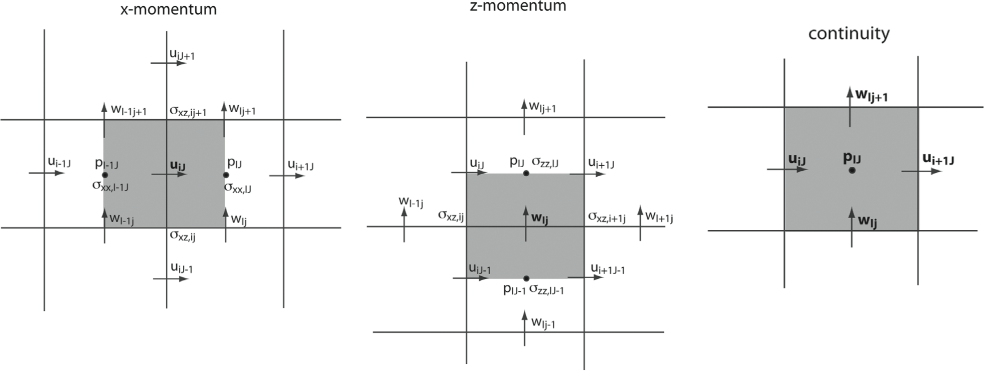
\includegraphics[width=0.7\textwidth]{figures/stagyy-discretization} \\
   {\scriptsize (P.~Tackley, Stagyy User Manual)}
  \end{center}

\end{frame}

\begin{frame}[fragile]\frametitle{StagYY: Performance Modeling}

{ \footnotesize
\begin{minipage}{0.45\textwidth}
\begin{block}{Iterated relaxation}
\begin{verbatim}
 - Update z-component of velocity
 - Exchange values of vz at boundaries
 
 - Compute pressure correction
 - Exchange correction values at boundaries
 - Apply pressure correction
 - Update velocity based on new pressure
 - Exchange boundary pressure and velocity
 
 - Update y-component of velocity
 - Exchange values of vy at boundaries

 - Update x-component of velocity
 - Exchange values of vx at boundaries
\end{verbatim}
\end{block}
\end{minipage}
\begin{minipage}{0.45\textwidth}
\begin{block}{All moments simultaneously}
\begin{verbatim}
 - Compute updates for all velocity components
 - Exchange boundary pressure and velocity

 - Compute correction for pressure p
 - Exchange correction values at boundaries
 - Apply pressure correction
 - Update velocity based  on new pressure
 - Exchange boundary pressure and velocity
   
   
   
   
  
   
\end{verbatim}
\end{block}
\end{minipage}
}


\end{frame}

% Optimization of boundary gather/scatter

\begin{frame}{StagYY}

  \begin{block}{GPU Data Handling}
  \begin{itemize}
   \item Fields on each multigrid hierarchy reside on GPU
   \item Stack-like mechanism for resident GPU data
  \end{itemize}
  \end{block}

  %\pause
  \begin{block}{GPU Boundary Value Handling}
  \begin{itemize}
   \item pTatin3d results: Pay attention to this
   \item MPI-like \texttt{gather} and \texttt{scatter} implemented
  \end{itemize}
  \end{block}

\begin{flushright}
  %\only<3>{ \vspace*{-4cm} \includegraphics[width=0.305\textwidth]{figures/gather} }
  %\only<4>{ \vspace*{-4cm} \includegraphics[width=0.305\textwidth]{figures/scatter} }
  \vspace*{-4cm} \includegraphics[width=0.305\textwidth]{figures/scatter}
\end{flushright}
  
\end{frame}





% Results (compare to CPU)

\begin{frame}{StagYY}

  \begin{block}{GPU Acceleration}
  \begin{itemize}
   \item One thread per residual entry
   \item Common kernel code path for CUDA and OpenCL
  \end{itemize}
  \end{block}

  %\pause
  \begin{block}{Observations}
   \begin{itemize}
    \item It works!
    %\pause
    \item Kernels fairly fast out-of-the-box!
   \end{itemize}
  \end{block}
  
\begin{center}
\begin{tabular}{|r|c|c|c|c|c|}
 \hline
 \textbf{nxtot=nytot=nztot}   & \textbf{GPU, CUDA, xyz} & \textbf{GPU, CUDA, classic}  &\textbf{Sequential} & \textbf{8 MPI ranks}  \\
 \hline
 \hline
 32                           &  0.27 &   0.28  &     0.36    &  0.08  \\
 64                           &  1.21 &   1.39  &     3.04    &  0.50  \\
 128                          &  5.66 &   5.33  &    24.4     &  4.4  \\
 256                          &  38.4 &  25.7   &    timeout  & 36.1  \\
 \hline
\end{tabular} \\
(Timings in seconds, Piz Daint after upgrade)
\end{center}
  
\end{frame}



% Profiling: Communication overhead!

\begin{frame}[fragile]\frametitle{StagYY: Performance Modeling}

  \begin{block}{GPU Profiling}
   \begin{itemize}
    \item 60-65 percent of GPU-time spent on PCI-Express transfer
    \item Checked: No unnecessary transfers, full bandwidth, etc.
   \end{itemize}
  \end{block}

  \begin{center}
\begin{tabular}{|r|c|c|c|c|}
 \hline
 \textbf{nxtot=nytot=nztot}   & \textbf{GPU, CUDA, xyz} & \textbf{GPU, CUDA, classic}  \\
 \hline
 \hline
 CUDA memcpy HtoD           &  39.03\% &  49.98\%  \\
 CUDA memcpy DtoH           &  20.78\% &  16.03\%  \\
 \hline
\end{tabular}
\end{center}


\end{frame}


%
% Performance Model: Figure out the problem
%
\begin{frame}[fragile]
\frametitle{StagYY: Performance Modeling}
  \begin{block}{Pitfall: GPUs are too fast for PCI-Express}
  \begin{itemize}
   \item Latest GPU peaks: 720 GB/sec from GPU-RAM, 16 GB/sec for PCI-Express
   \item 40x imbalance (!)
  \end{itemize}
  \end{block}

  %\pause
  \begin{center} \vspace*{-0.8cm}
    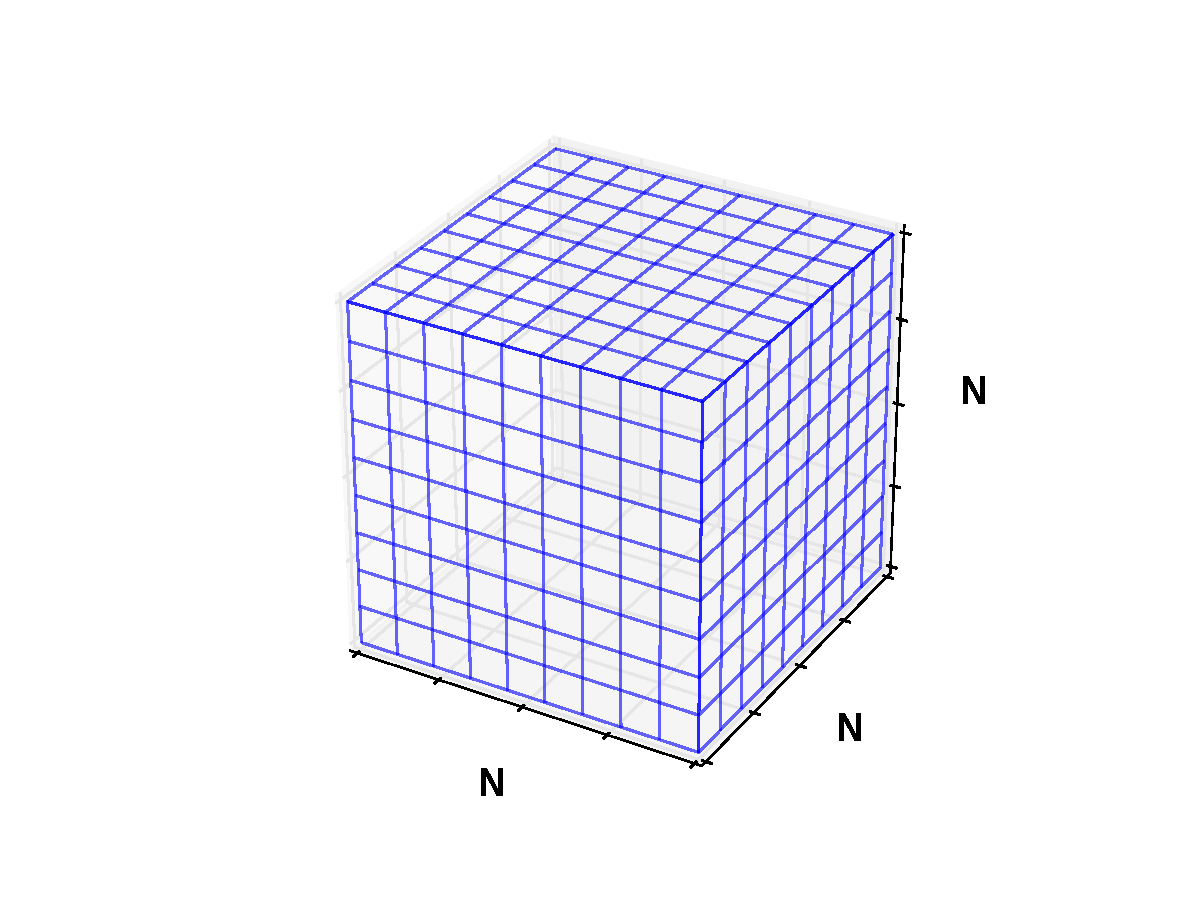
\includegraphics[width=0.4\textwidth]{figures/cube-discretization.pdf}
  \end{center}

  %\pause
  \vspace*{-1.0cm}
   \begin{block}{Compute vs. Communication}
  \begin{itemize}
   \item Take $N=512$, so each field consumes 1 GB of GPU RAM
   \item Boundary communication: $2 \times 6 \times N^2$: 31 MB
   %\pause
   \item Time to process field on GPU: 1.4 ms
   %\pause
   \item Time to load ghost data: \textbf{1.9 ms (!!)}
  \end{itemize}
  \end{block}

\end{frame}




%%
%% Summary
%%

\begin{frame}{Summary}

 \begin{block}{GPU-SpMV in pTatin3d}
   \begin{itemize}
    \item 166 GFLOPs in GPU kernel achieved
    \item One thread per Q2 quadrature point
    \item Overhead due to host-device communication significant
   \end{itemize}
 \end{block}

 %\pause
 \begin{block}{GPU-assisted Multigrid in StagYY}
   \begin{itemize}
    \item Residual evaluation and relaxations
    \item Reduced boundary data transfer between host and GPU (cf.~gather and scatter)
    \item Heavily PCI-Express bandwidth limited
   \end{itemize}
 \end{block}

 %\pause
 \begin{block}{General Conclusions}
   \begin{itemize}
    \item Starvation of modern GPUs for multigrid when attached via PCI-Express 
    \item Kernel-level GPU integration insufficient for multigrid purposes
   \end{itemize}
 \end{block}

\end{frame}

